\documentclass[a4paper,10pt,titlepage,oneside,openright]{book}
	 \textheight = 24cm
	 \textwidth = 18cm
	 \topmargin = -1cm
	 \oddsidemargin = -1cm
	 
%\input{../../../header-apuntes.tex} %Ponemos ruta de la cabecera
\setcounter{secnumdepth}{3} % Para enumerar hasta subsubsection
\setcounter{tocdepth}{3} % Para enumerar hasta subsubsection 
 
\usepackage{indentfirst} % Paquete para iniciar el primer párrafo de una sección con sangría
\usepackage[utf8]{inputenc}
\usepackage[none]{hyphenat} %Paquete para indicar que no separe las palabras
\usepackage{graphicx} %Paquete para incluir imágenes
\usepackage{fancyhdr} %Paquete para modificar los pies de página y encabezados
\usepackage{listings} %Paquete para poner código de programación
\usepackage{color} %Paquete para definir los colores
\usepackage[hidelinks]{hyperref} %Paquete para que el índice tenga referencia
\usepackage{wrapfig} %Paquete para poner las imágenes con el texto en un lado.
\usepackage{multicol} %Paquete para poner texto en dos columnas
\usepackage{enumitem} %Paquete para poner en enumerate: 1.2, 1.3,...
\usepackage[nottoc]{tocbibind} %Paquete para incluir la bibliografía en el índice
\usepackage{colortbl} %Paquete para poner colores en las celdas
\usepackage{tocloft} %Paquete para personalizar el índice
\usepackage{textcomp} %Paquete para insertar símbolos raros
\usepackage{amssymb} %Paquete para insertar flechas raras
\usepackage{enumitem} %Paquete pare personalizar los enumerate
%\usepackage{kbordermatrix} %Parquete para poner bordes en las matrices

\definecolor{blue-violet}{rgb}{0.54,0.17,0.89}
\definecolor{darkcerulean}{rgb}{0.03, 0.27, 0.49}
\definecolor{ceruleanblue}{rgb}{0.16, 0.32, 0.75}
\definecolor{dkgreen}{rgb}{0,0.6,0}
\definecolor{gray}{rgb}{0.5,0.5,0.5}
\definecolor{mauve}{rgb}{0.58,0,0.82}
\definecolor{gray97}{gray}{.97}
\definecolor{gray75}{gray}{.75}
\definecolor{gray45}{gray}{.45}

\lstset{frame=Ltb,
  language=Python,
  framerule=0pt,
  aboveskip=0.5cm,
  framextopmargin=3pt,
  framexbottommargin=3pt,
  framexleftmargin=0.4cm,
  framesep=0pt,
  rulesep=.4pt,
  backgroundcolor=\color{gray97},
  rulesepcolor=\color{black},
  %
  stringstyle=\color{mauve},
  showstringspaces = false,
  basicstyle=\small\ttfamily,
  commentstyle=\color{gray45},
  keywordstyle=\color{darkcerulean},
  %
  numbers=left,
  numbersep=15pt,
  numberstyle=\tiny,
  numberfirstline = false,
  breaklines=true,
  escapeinside=||,
  %
  literate={«}{{\guillemotleft}}1
           {»}{{\guillemotright}}1
           {é}{{\'e}}1
           {í}{{\'i}}1
           {ó}{{\'o}}1
           {ú}{{\'u}}1
           {á}{{\'a}}1
           {ñ}{{\~n}}1
           {Ñ}{{\~N}}1
           {¿}{{?`}}1
}

% minimizar fragmentado de listados
\lstnewenvironment{listing}[1][]
{\lstset{#1}\pagebreak[0]}{\pagebreak[0]}

\renewcommand{\contentsname}{Índice}
\renewcommand{\partname}{TEMA}
\renewcommand{\chaptername}{Tarea}
\renewcommand{\thesection}{\arabic{section}}
\renewcommand{\listtablename}{Índice de tablas}
\renewcommand{\tablename}{Tabla}
\renewcommand{\figurename}{Figura}
\renewcommand{\bibname}{Bibliografía}
% \renewcommand{\cftsecfont}{\bfseries} % Poner las secciones en negrita en el índice

% Personalización del itemize
\renewcommand{\labelitemi}{\textendash}
\renewcommand{\labelitemii}{\textperiodcentered}
\renewcommand{\labelitemiii}{\textasciicircum}

	
\graphicspath{ {images/} } %Indicamos la carpeta donde están las imágenes

\newcounter{ejemplo} % Contador para los ejemplos
%\addtocounter{ejemplo}{1} % Sumamos 1

\newcommand{\master}{M. Big Data \& Business Analytics}
\newcommand{\module}{Módulo V: Inteligencia de Negocio y Visualización}


\begin{document}
%--------------------------------------------------------------------
\thispagestyle{empty}
\begin{figure}[h]

\includegraphics[scale=0.3]{logo-imf.png} \hspace{80mm}

\includegraphics[scale=0.25]{logo-ucjc.png}
\centering
\end{figure}

\vspace{5mm}

\begin{center}
\rule{150mm}{0.1mm} \\
\vspace{5mm}
\begin{Huge}
 \textsc{Máster en \\ ~ \\ Big Data \& Business Analytics}
\end{Huge}
\vspace{5mm} \\
\rule{150mm}{0.5mm}

\vspace{20mm}

\begin{huge}
  \textsc{Módulo V: \\ Inteligencia de Negocio y \\ Visualización} \\ \vspace{15mm}
\end{huge}

\begin{LARGE}
 Documentación del caso práctico\\ \vspace{5mm}
 {\large 22 de Octubre del 2018}
\end{LARGE}

\vspace{25mm}

\begin{Large}
\begin{center}
\begin{tabular}{ccc}
\textbf{Autor} \\
José María Sánchez Salas \\
\textit{josemaria.sanchezsalas@gmail.com}
\end{tabular}
\end{center}
\end{Large}
\end{center}
%--------------------------------------------------------------------
\newpage
\thispagestyle{empty}
\section*{}
\newpage

\thispagestyle{empty}

\tableofcontents
\addtocontents{toc}{\textbf{\module}}

\newpage
\thispagestyle{empty}
\section*{}
\newpage

\pagestyle{fancy}
\fancyhf{}
\fancyhead[LE,RO]{\module}
\fancyhead[RE,LO]{\master}
\fancyfoot[CE,CO]{\thepage}

% \lhead[]{} - \chead[]{} - \rhead[]{}
\renewcommand{\headrulewidth}{0.5pt} % --> Definimos el grosor de la línea
\renewcommand{\footrulewidth}{0.5pt}

%--------------------------------------------------------------------
\medskip
\section{Introducción}
Este documento contiene la explicación de mi solución propuesta al caso práctico del {\module}, del {\master} impartido por IMF Business School. 

% El documento contiene dos secciones: uno para cada uno de los ejercicios del caso práctico. En cada ejercicio, se muestra previamente su enunciado y posteriormente la solución propuesta.



%--------------------------------------------------------------------
\medskip
\section{Enunciado}
El departamento antifraude de una compañía de Mystery Shopping desea hacer un seguimiento y
analizar la información relativa a las encuestas que realiza en los distintos centros de sus clientes. Para
ello, el cliente solicita:

\begin{itemize}
    \item Un análisis y diseño del Data Warehouse que daría respuesta a los usuarios analíticos del
departamento antifraude, suponiendo que los usuarios aún no tienen claro el tipo de análisis
que quieren realizar.
    \item Partiendo del análisis y diseño previo realizado y usando Pentaho Data Integration, se debe
realizar la implementación del proceso ETL con el objetivo de:
    \begin{itemize}
        \item Identificar y extraer los datos de las fuentes.
        \item Procesar los datos y aplicar procesos de limpieza y calidad del dato.
        \item Generar y cargar los datos en el modelo físico de estrella identificado en la fase de diseño.
    \end{itemize}

    \item Posteriormente, partiendo del análisis y diseño previo realizado y conociendo ya la tecnología
seleccionada, en este caso Pentaho Business Analytics, ha de realizarse una implementación
ágil del modelo multidimensional.
\end{itemize}


El objetivo en este caso es la implementación del modelo multidimensional sobre diseño del Data
Warehouse que daría respuesta a los usuarios analíticos del departamento antifraude, suponiendo que los
usuarios aún no tienen claro el tipo de análisis que quieren realizar.




%--------------------------------------------------------------------
\medskip
\section{Solución}



%--------------------------------------------------------------------
\medskip
\subsection{Análisis de fuentes}
\label{01}
En esta sección se va a realizar el análisis de las fuentes de las que se dispone en este caso práctico. La sección está dividida en dos secciones: la primera de ellas se hace una descripción global de las fuentes mientras que en la segunda se hace una descripción detallada de los campos que contienen cada una de las fuentes.


%--------------------------------------------------------------------
\medskip
\subsubsection{Descripción global de las fuentes}
Para este problema se nos presenta una única fuente: un fichero en formato CSV que contiene la información de todos las encuestas registradas por la compañía Mystery Shopping. Este fichero CSV contiene los siguientes campos:


%--------------------------------------------------------------------
\medskip
\subsubsection{Descripción en detalle de cada campo}

\begin{itemize}
 \item \texttt{COD\_LOC}. Se trata del código de centro en el que se realizó la encuesta. Es un campo alfanumérico y único que identifica al centro.
 \item \texttt{NOMBRE\_LOC}. Se trata del nombre del centro al que corresponde el campo anterior. Es un campo alfanumérico.
 \item \texttt{CP}. Corresponde con el código postal del centro y es un campo numérico.
 \item \texttt{POBLACION}. Corresponde con la población asociada al código postal y en el que se ubica el centro. Se trata de un campo alfanumérico.
 \item \texttt{OFICINA}. Se trata de la oficina a la que está asignada el centro. Se trata de un campo alfanumérico.
 \item \texttt{PROVINCIA}. Provincia a la que pertenece la población del centro. Es un campo alfanumérico.
 \item \texttt{COD\_PROY}. Código del proyecto al que se hace la encuesta. Es un campo alfanumérico.
 \item \texttt{ID\_EVALUACION}. Código identificativo de la evaluación, es un campo numérico y único.
 \item \texttt{FECHA DE EJECUCION}. Se trata de la fecha en la que se realizó la encuesta. Es un campo de tipo fecha.
 \item \texttt{COD\_AUDITOR}. Código del auditor que realizó la encuesta. Se trata de un campo alfanumérico y único.
 \item \texttt{RESULTADO}. Se trata del resultado de la encuesta realizada. Es un campo numérico decimal entre 0 y 1.
 \item \texttt{TITULO\_CUESTIONARIO}. Título que tiene asociado el cuestionario que se ha realizado. Se trata de un campo alfanumérico y único.
\end{itemize}

%--------------------------------------------------------------------
\medskip
\subsection{Análisis funcional y diagrama de arquitectura de flujo de datos}

%--------------------------------------------------------------------
\medskip
\subsection{¿Qué arquitectura de referencia usaría? Justifique la respuesta}

%--------------------------------------------------------------------
\medskip
\subsection{¿Qué tecnología OLAP usaría? Justifique la respuesta}

% %--------------------------------------------------------------------
\medskip
\subsection{Si se utiliza ROLAP, ¿cuál de estos dos modelos se ajustaría mejor: modelo de estrella o el de copo de nieve?}
\label{05}
La sencillez de la estructura de la fuente de datos supone que el modelo que mejor se ajustaría es el modelo de estrella, ya que utilizar un modelo de copo de nieve supondría añadir complejidad al sistema. En la Figura \ref{07-image} de la sección \ref{07} se muestra el modelo de estrella que se va a emplear para esta solución.

% %--------------------------------------------------------------------
\medskip
\subsection{Si se utiliza ROLAP, hay que identificar y justificar si existe algún proceso de desnormalización de información que se deba realizar}
Analizando los datos almacenados en la fuente de datos, se puede observar que no hay una normalización en los datos. Además, dado que se trata de encuestas que realiza la empresa, el sistema que proporciona la fuente de datos no es un sistema OLTP en el que se necesite rendimiento procesando pequeñas transacciones, por lo que la fuente de datos no está normalizada y, por consecuencia, no es necesario aplicar un proceso de desnormalización de la información.

% %--------------------------------------------------------------------
\medskip
\subsection{Si se utiliza ROLAP, se debe incluir un diseño conceptual a modo explicativo junto con un diagrama}

% %--------------------------------------------------------------------
\medskip
\subsection{Si se utiliza ROLAP, se debe incluir un diseño modelo lógico}
\label{08}
Lo primero que se ha de hacer para realizar el diseño de un modelo lógico es identificar las dimensiones. Las \textbf{dimensiones} para este problema son: \texttt{Cliente}, \texttt{Proyecto}, \texttt{Auditor} y \texttt{Evaluación}. \\

Seguidamente, identificar los hechos. Los \textbf{hechos} son los resultados obtenidos en las encuestas. \\

Y por último, definir las métricas. Las \textbf{métricas} directas que se pueden definir son: \textit{Resultado final de la encuestas, cuya función de agregación sería la suma}.\\

Una vez definidas las dimensiones, hechos y métricas, el siguiente paso es jerarquizar la información. Así pues, la jerarquización para todas las dimensiones anteriores es:
\begin{itemize}
 \item \texttt{Cliente}. Esta dimensión tiene dos jerarquías:
 \begin{itemize}
  \item \texttt{Local}, cuyos niveles son: \texttt{Código Local} y \texttt{Nombre Local}.
  \item \texttt{Localización}, cuyos niveles son: \texttt{Provincia} y \texttt{Oficina}. A su vez, el nivel de \texttt{Provincia}, tiene los siguientes niveles:
  \begin{itemize}
   \item \texttt{Población}.
   \item \texttt{Código Postal}.
  \end{itemize}

 \end{itemize}

 \item \texttt{Proyecto}. Esta dimensión solamente tiene la jerarquía \texttt{Proyecto} cuyo nivel es \texttt{Código Proyecto}.
 \item \texttt{Auditor}. Esta dimensión solamente tiene la jerarquía \texttt{Auditor} cuyo nivel es \texttt{Código Auditor}.
 \item \texttt{Evaluación}. Esta dimensión solamente tiene la jerarquía \texttt{Evaluación} con los siguientes niveles:
\begin{itemize}
 \item \texttt{Evaluación}.
 \item \texttt{Título}.
 \item \texttt{Fecha}.
\end{itemize}
\end{itemize}

Así pues, en la Figura \ref{08-image} se muestra el modelo lógico para el Data Mart Mistery Shopping.

\begin{figure}[!th]
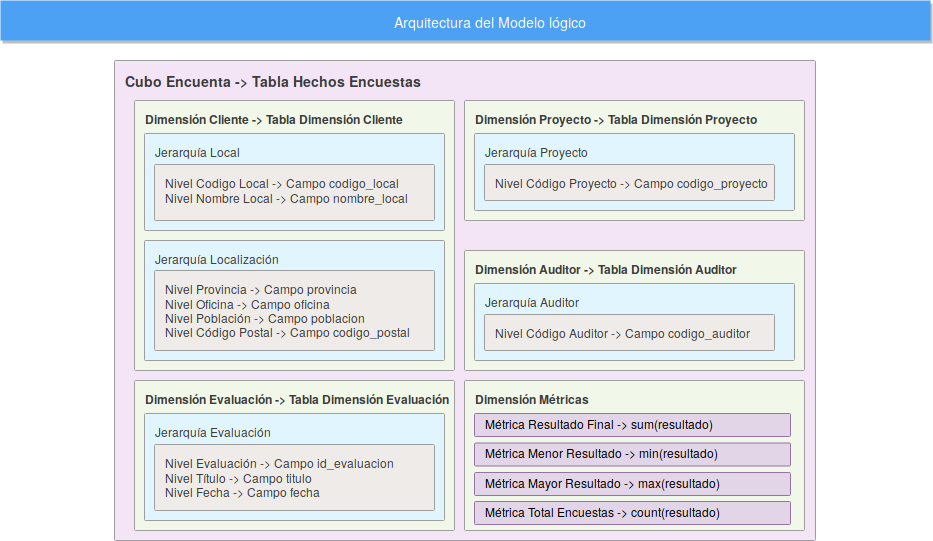
\includegraphics[scale=0.5]{08.png}
\centering
\caption{Modelo lógico para el Data Mart Mistery Shopping.}
\label{08-image}
\end{figure}

% %--------------------------------------------------------------------
\medskip
\subsection{Si se utiliza ROLAP, se debe incluir un diseño modelo físico}

% %--------------------------------------------------------------------
\medskip
\subsection{Realizar la implementación del proceso ETL para generar y poblar el modelo multidimensional diseñado en los apartados anteriores}
Para la realización de este apartado, se ha hecho uso de la herramienta Pentaho y se parte del JOB/Trabajo global \texttt{Global\_IMF\_def.kjb} proporcionado en el módulo de este caso práctico y que se encuentra situado en la carpeta \texttt{src/} y cuya estructura se muestra en la Figura \ref{Global_IMF}. En la carpeta \texttt{src/} se encuentran todos los ficheros fuente utilizados para el proceso ETL.

\begin{figure}[!th]
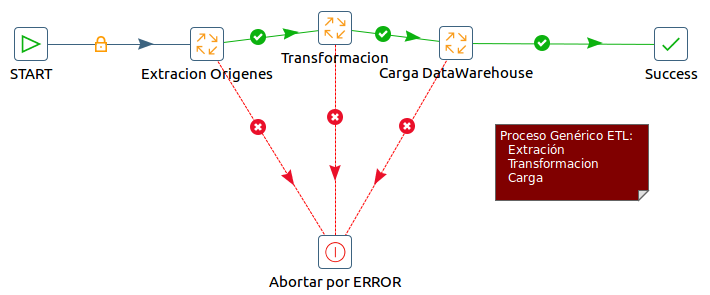
\includegraphics[scale=0.5]{Global_IMF.png}
\centering
\caption{Estructura del trabajo \texttt{Global\_IMF\_def}.}
\label{Global_IMF}
\end{figure}

A continuación se van a explicar en detalle cada uno de los trabajos en los que se divide este trabajo global:


%--------------------------------------------------------------------
\medskip
\subsubsection{Extracción Orígenes}
La estructura general de este trabajo se encuentra en el fichero \texttt{Global\_Extraccion.kjb} y se muestra en la Figura \ref{Global_Extraccion}.

\begin{figure}[!th]
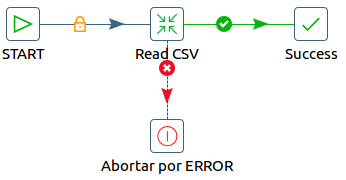
\includegraphics[scale=0.5]{Global_Extraccion.png}
\centering
\caption{Estructura del trabajo \texttt{Global\_Extraccion}.}
\label{Global_Extraccion}
\end{figure}

En este trabajo lo único que se hace es leer los datos que vienen proporcionados por la fuente de datos descrita en la sección \ref{01} y volcarlos todos en una tabla que servirá de entrada para el trabajo de Transformación explicado en la sección \ref{Transformacion}. Esto se hace a través de una transformación de Pentaho y que se encuentra en el fichero \texttt{Read\_CSV.ktr} y cuya estructura se muestra en la Figura \ref{Read_CSV}.

\begin{figure}[!th]
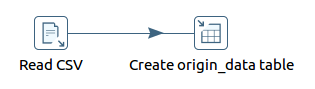
\includegraphics[scale=0.5]{Read_CSV.png}
\centering
\caption{Estructura de la transformación \texttt{Read\_CSV}.}
\label{Read_CSV}
\end{figure}


\newpage
%--------------------------------------------------------------------
\medskip
\subsubsection{Transformación}
\label{Transformacion}
La estructura general de este trabajo se encuentra en el fichero \texttt{Global\_Transformacion.kjb} y se muestra en la Figura \ref{Global_Transformacion}.

\begin{figure}[!th]
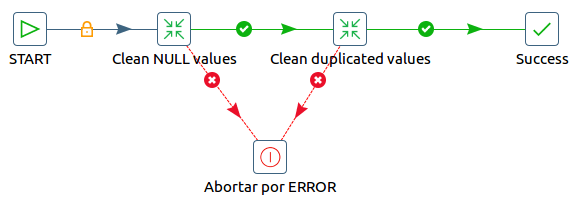
\includegraphics[scale=0.5]{Global_Transformacion.png}
\centering
\caption{Estructura del trabajo \texttt{Global\_Transformacion}.}
\label{Global_Transformacion}
\end{figure}

En este proceso se realizan dos transformaciones: una para eliminar aquellos registros con valores nulos y otra para eliminar aquellos registros que contengan claves primarias duplicadas. A continuación se explica cada una con mayor detalle:


%--------------------------------------------------------------------
\medskip
\subsubsection*{Eliminación valores nulos}
Como se definió en el modelo físico en la sección \ref{09}, en todas las tablas existe un campo como clave primaria (\texttt{PK}) y por definición, este campo no puede ser nulo. Por lo que se van a eliminar aquellos registros que contengan en alguno de los campos \texttt{PK} un valor \texttt{NULL}. Para ello, se hace uso de la transformación \texttt{Clean\_NULL\_values.ktr} y cuya estructura se muestra en la Figura \ref{NULL_values}.

\begin{figure}[!th]
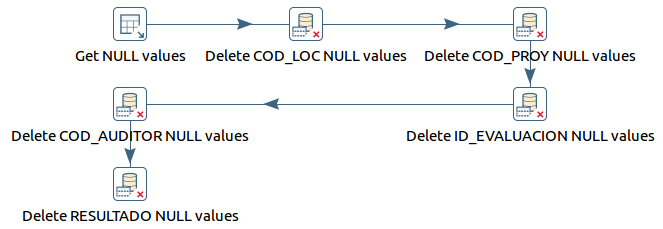
\includegraphics[scale=0.5]{Clean_NULL_values.png}
\centering
\caption{Estructura del trabajo \texttt{Clean\_NULL\_values}.}
\label{NULL_values}
\end{figure}

Además, para obtener estos registros, se hace uso de la siguiente sentencia SQL:
\lstinputlisting{code/SELECT_NULL_VALUES.sql}

Importante destacar que aunque el campo \texttt{RESULTADO} es una clave primaria, se trata del campo que se quiere analizar por el departamento antifraude, por lo que este tampoco puede ser nulo.


\newpage
%--------------------------------------------------------------------
\medskip
\subsubsection*{Eliminación claves primarias duplicadas}
Por definición, un valor de un campo que es clave primaria (\texttt{PK}) es único, ya que identifica de manera unívoca a cada registro. Pues siguiendo esta definición, se tiene que asegurar que en la fuente de datos no vienen registros distintos que hacen referencia a la misma clave primaria, lo cual duplicaría la clave primaria. Por ejemplo, supongamos que tenemos los siguientes registros, donde \texttt{codigo\_local} es la clave primaria:

\begin{center} 
\begin{table}[!th]
\begin{tabular}{|c|c|} \hline
\texttt{codigo\_local} & \texttt{nombre\_local} \\ \hline
1 & Pepito \\ \hline
1 & Menganito \\ \hline 
\end{tabular}
\centering
\end{table}
\end{center}

En este caso, si se intentan insertar ambos registros en la tabla \texttt{CLIENTE}, saltará un error diciendo que el valor \texttt{1} está duplicado. Como no podemos quedarnos con uno, porque no sabemos cuál es el correcto y cuál el erróneo, tenemos que eliminar ambos.\\

Siguiendo esta filosofía, se hace la transformación \texttt{Clean\_duplicated\_values.ktr} y cuya estructura se muestra en la Figura \ref{duplicated_values}.

\begin{figure}[!th]
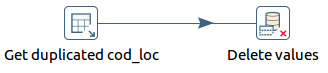
\includegraphics[scale=0.5]{Clean_duplicated_values.png}
\centering
\caption{Estructura del trabajo \texttt{Clean\_duplicated\_values}.}
\label{duplicated_values}
\end{figure}

Además, para obtener estos registros, se hace uso de la siguiente sentencia SQL:
\lstinputlisting{code/SELECT_DUPLICATED_VALUES.sql}




%--------------------------------------------------------------------
\medskip
\subsubsection{Carga DataWarehouse}
Por último, tras realizar las transformaciones hay que realizar la carga del DataWarehouse. Para ello, se hace uso del trabajo \texttt{Global\_Carga.kjb} y cuyo esquema se muestra en la Figura \ref{Global_Carga}.

\begin{figure}[!th]
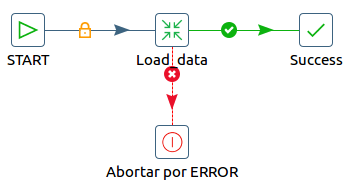
\includegraphics[scale=0.5]{Global_Carga.png}
\centering
\caption{Estructura del trabajo \texttt{Global\_Carga}.}
\label{Global_Carga}
\end{figure}

\newpage
Este trabajo lo que hace es crear cada una de las tablas definidas en la sección \ref{09} con los datos que ya han sido transformados. Para ello, hace uso de la transformación \texttt{Load\_data} cuyo estructura se muestra en la Figura \ref{Load_data}


\begin{figure}[!th]
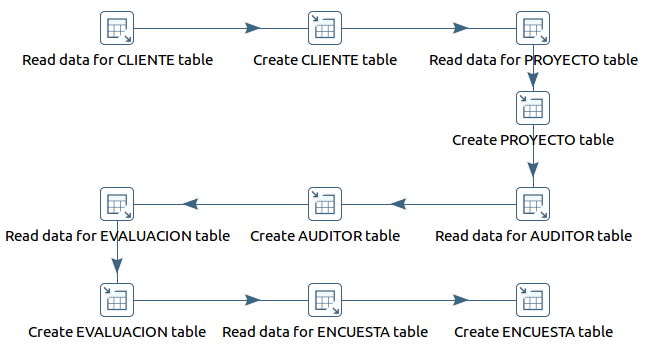
\includegraphics[scale=0.5]{Load_data.png}
\centering
\caption{Estructura de la transformación \texttt{Load\_data}.}
\label{Load_data}
\end{figure}

Las sentencias SQL necesarias para crear cada una de las tablas se muestran a continuación:
\lstinputlisting{code/CREATE_TABLES.sql}

Es importante destacar aquí que en la creación de la tabla \texttt{ENCUESTA} no se definen los campos \texttt{CLIENTE}, \texttt{PROYECTO}, \texttt{AUDITOR} y \texttt{EVALUACION} como claves foráneas (\texttt{FK}) porque al intentar lanzar el proceso entero y borrar todas las tablas con un \texttt{TRUNCATE} como hace Pentaho, da error por las restricciones de clave foránea, incluso si se pone \texttt{ON DELETE SET NULL} en la definición sigue dando el mismo error. Sin embargo, al rellenar la tabla, se hace uso de las claves primarias definidas.

% %--------------------------------------------------------------------
\medskip
\subsection{Implementación de modelo multidimensional diseñado mediante los puntos anteriores}

% %--------------------------------------------------------------------
\medskip
\subsection{Análisis de modelo}





%--------------------------------------------------------------------
% \medskip
% \section{Conclusiones}

















\end{document}
